\documentclass[letter,10pt, twocolumn]{article}
\usepackage[utf8]{inputenc}
\usepackage{graphicx}
\usepackage[english]{babel} 
\usepackage{lipsum}
\usepackage{multicol}
\usepackage{geometry}
\geometry{
 left=20mm, right=20mm,
 top=20mm, bottom=20mm,
 }
 \usepackage{abstract}
\renewcommand{\abstractnamefont}{\normalfont\Large\bfseries}
\renewcommand{\abstracttextfont}{\normalfont\Huge}

\renewcommand{\thesection}{\Roman{section}} 
\renewcommand{\thesubsection}{\thesection.\Roman{subsection}}

\title{Evaluation of the unbinding kinetics of Mineralocorticoid (MR) receptor steroid agonist Cortisol (COL) , Aldosterone (AS4), and Progesteron (STR) ligands using Molecular Dynamics (MD) and Monte Carlo (MC) simulations}

\author{Sebastian Aguilera Novoa}
\date{April 14, 2023}



\begin{document}

%\maketitle

\twocolumn[
  \begin{@twocolumnfalse}
    \maketitle
    \begin{abstract}
    \normalsize
    asdasdasd
    \vspace{20pt}
    \end{abstract}
  \end{@twocolumnfalse}
]



\section{Introduction}


Is wildly known the important role of the mineralocorticoid hormone aldosterone in the cardiovascular system, in particular in the effects that have in the kidney. Nevertheless, several researches have demonstrated the importance of this hormone \cite{book-MR_AS4, MR-as4_importance}


\cite{Activating_Mineralocorticoid}


\begin{figure}[h]
%\centering
\hspace*{-25pt}   
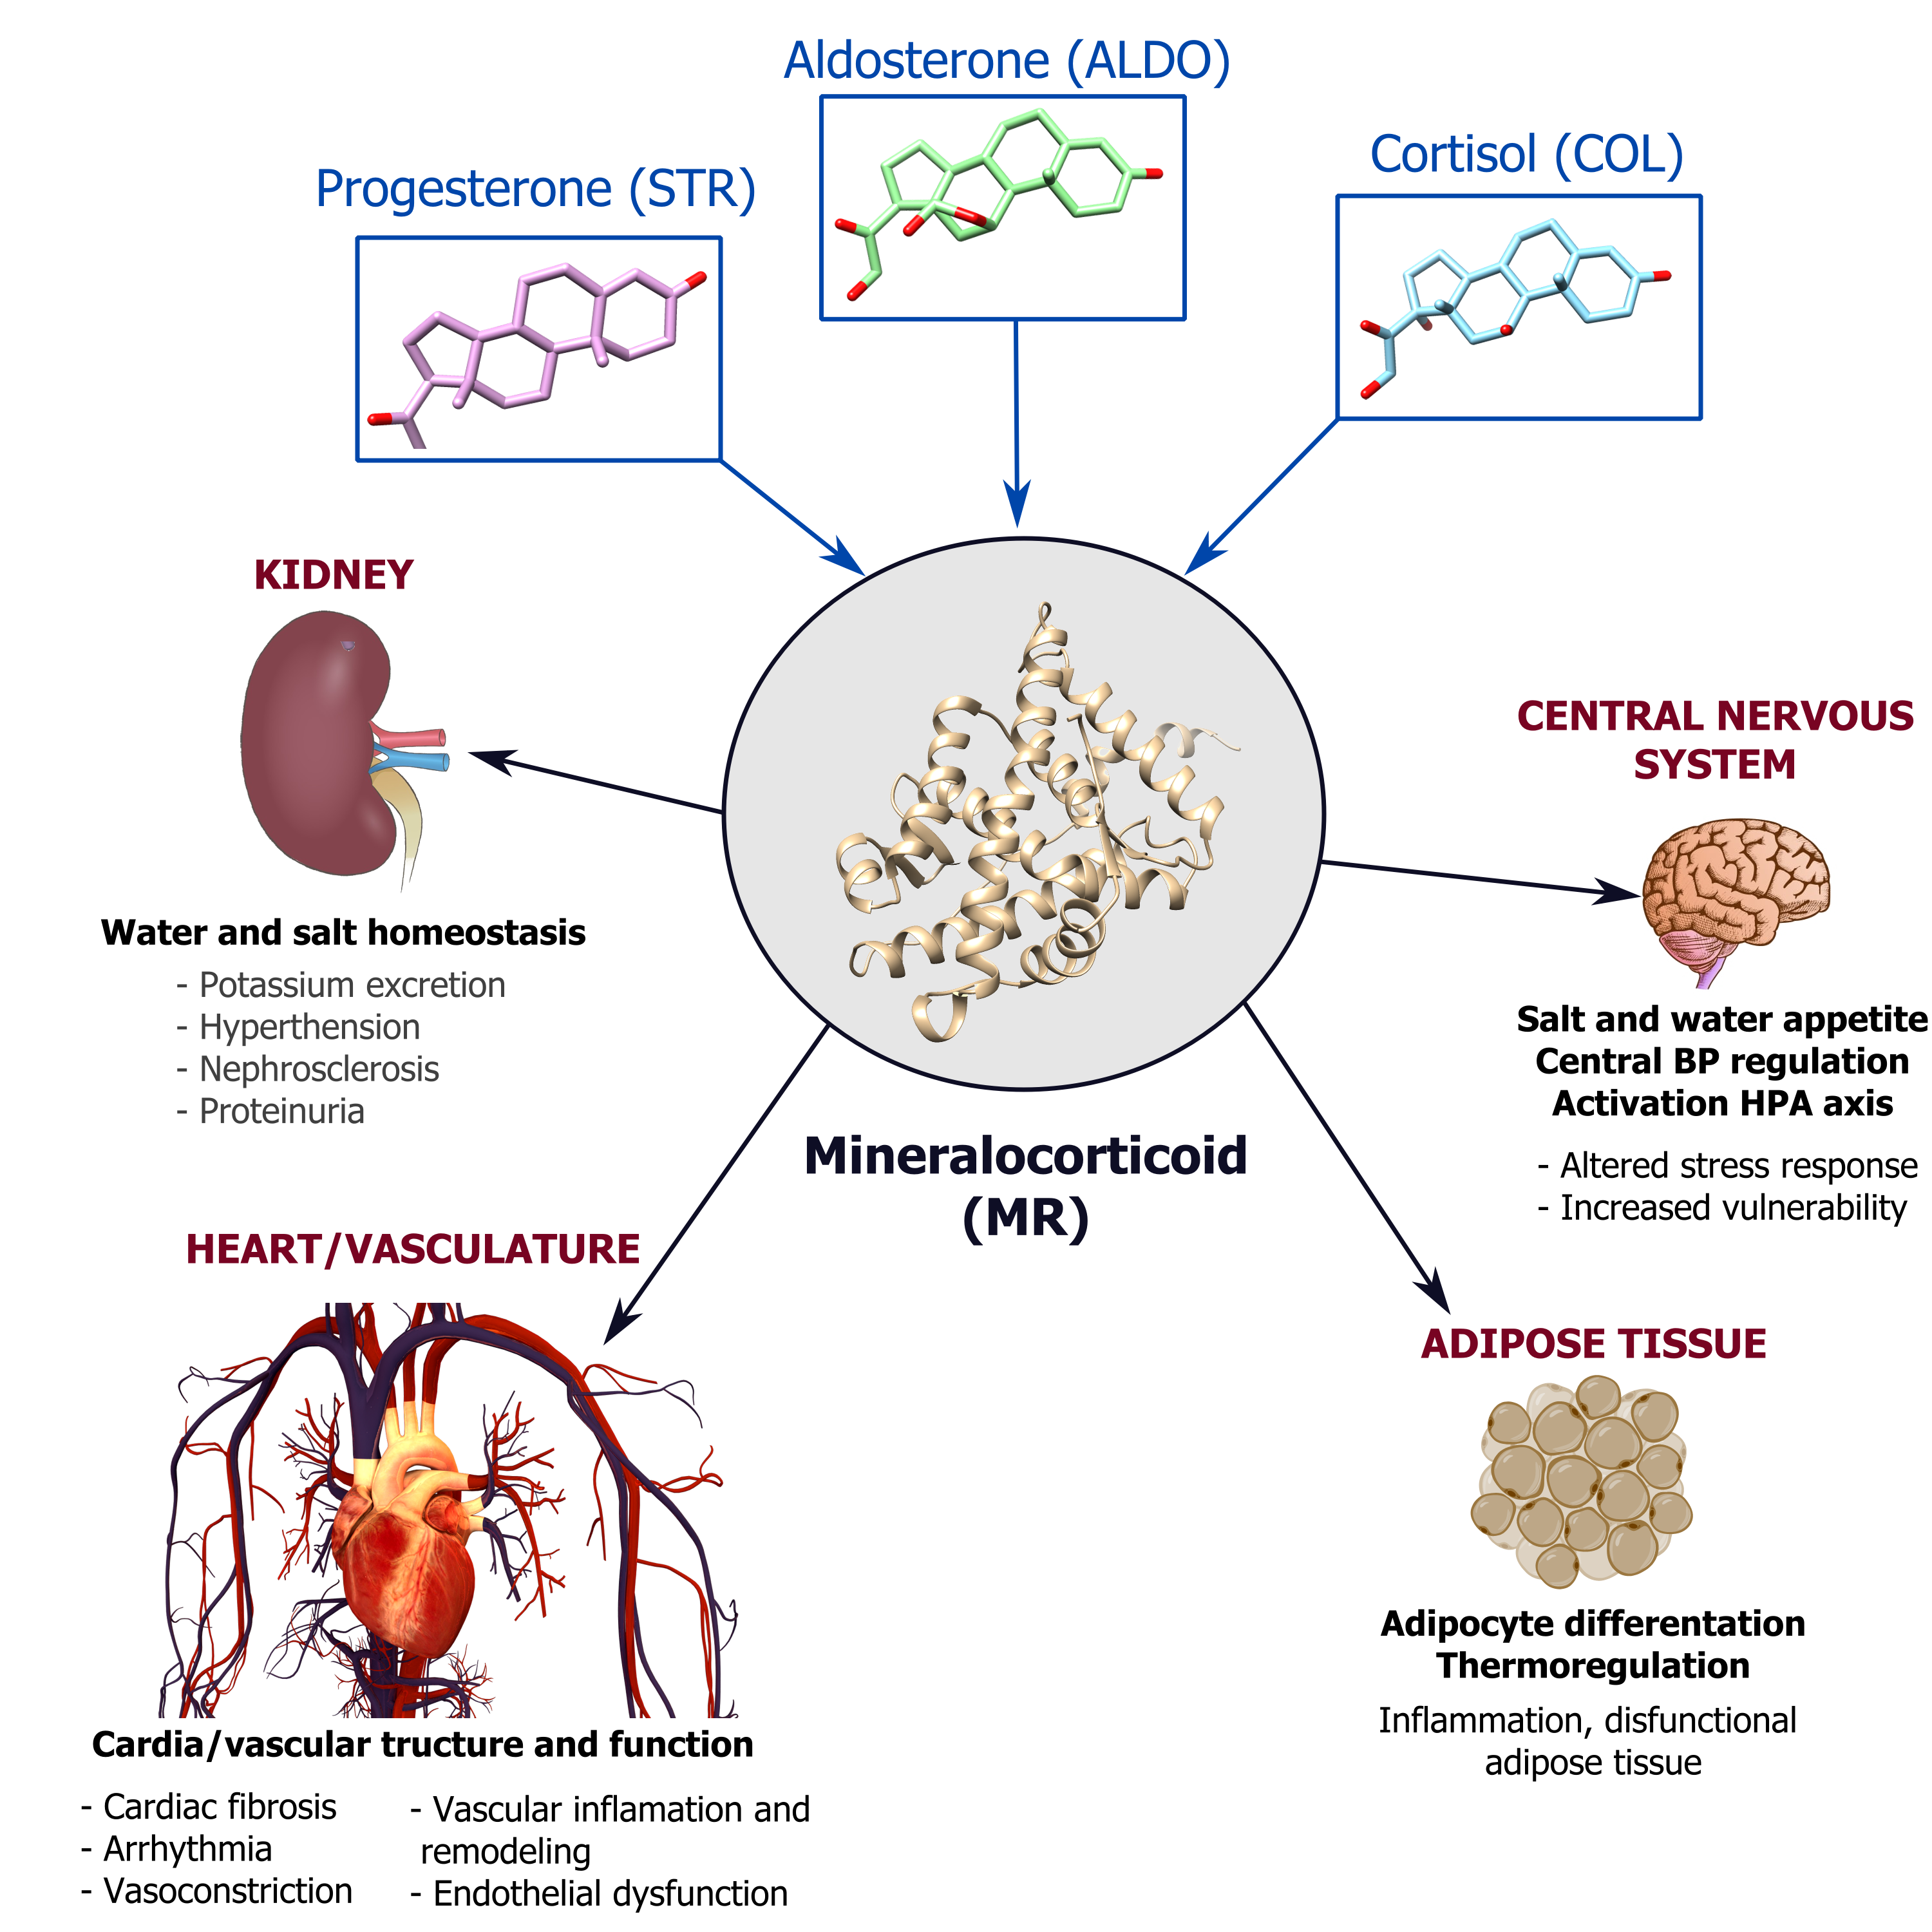
\includegraphics[scale=0.35]{MR-AS4-COL.png}
\caption{Mineralocorticoid/aldosterone receptor impact on health. \textit{Image taken and adapted from \cite{book-MR_AS4}.}}
\label{MR_functions}
\end{figure}




\section{Methods}

Selection of the best method to simulate the system, description of the simulation methods and how are we analyzing the date, since the MD simulations have a sense of time while the MC simulations does not, pyEMMA.

LiBEla 
\cite{libela}


Amber and LiGaMD
\cite{amber}

\cite{ligamd_Miao, ligamd2}

\cite{pyemma}

why MC and MD, what software are we using?


\section{Results and Discussion}

Select images of interest and explain them


\section{Conclusion}

What is possible to conclude from each simulation and how can it be explain from chemistry and physics

\begin{itemize}

\item 

\end{itemize}


\clearpage
\onecolumn{
\bibliography{../references}
\bibliographystyle{unsrt.bst}
%\nocite{*}
}

\end{document}
